\begin{figure}[!t]
\centering
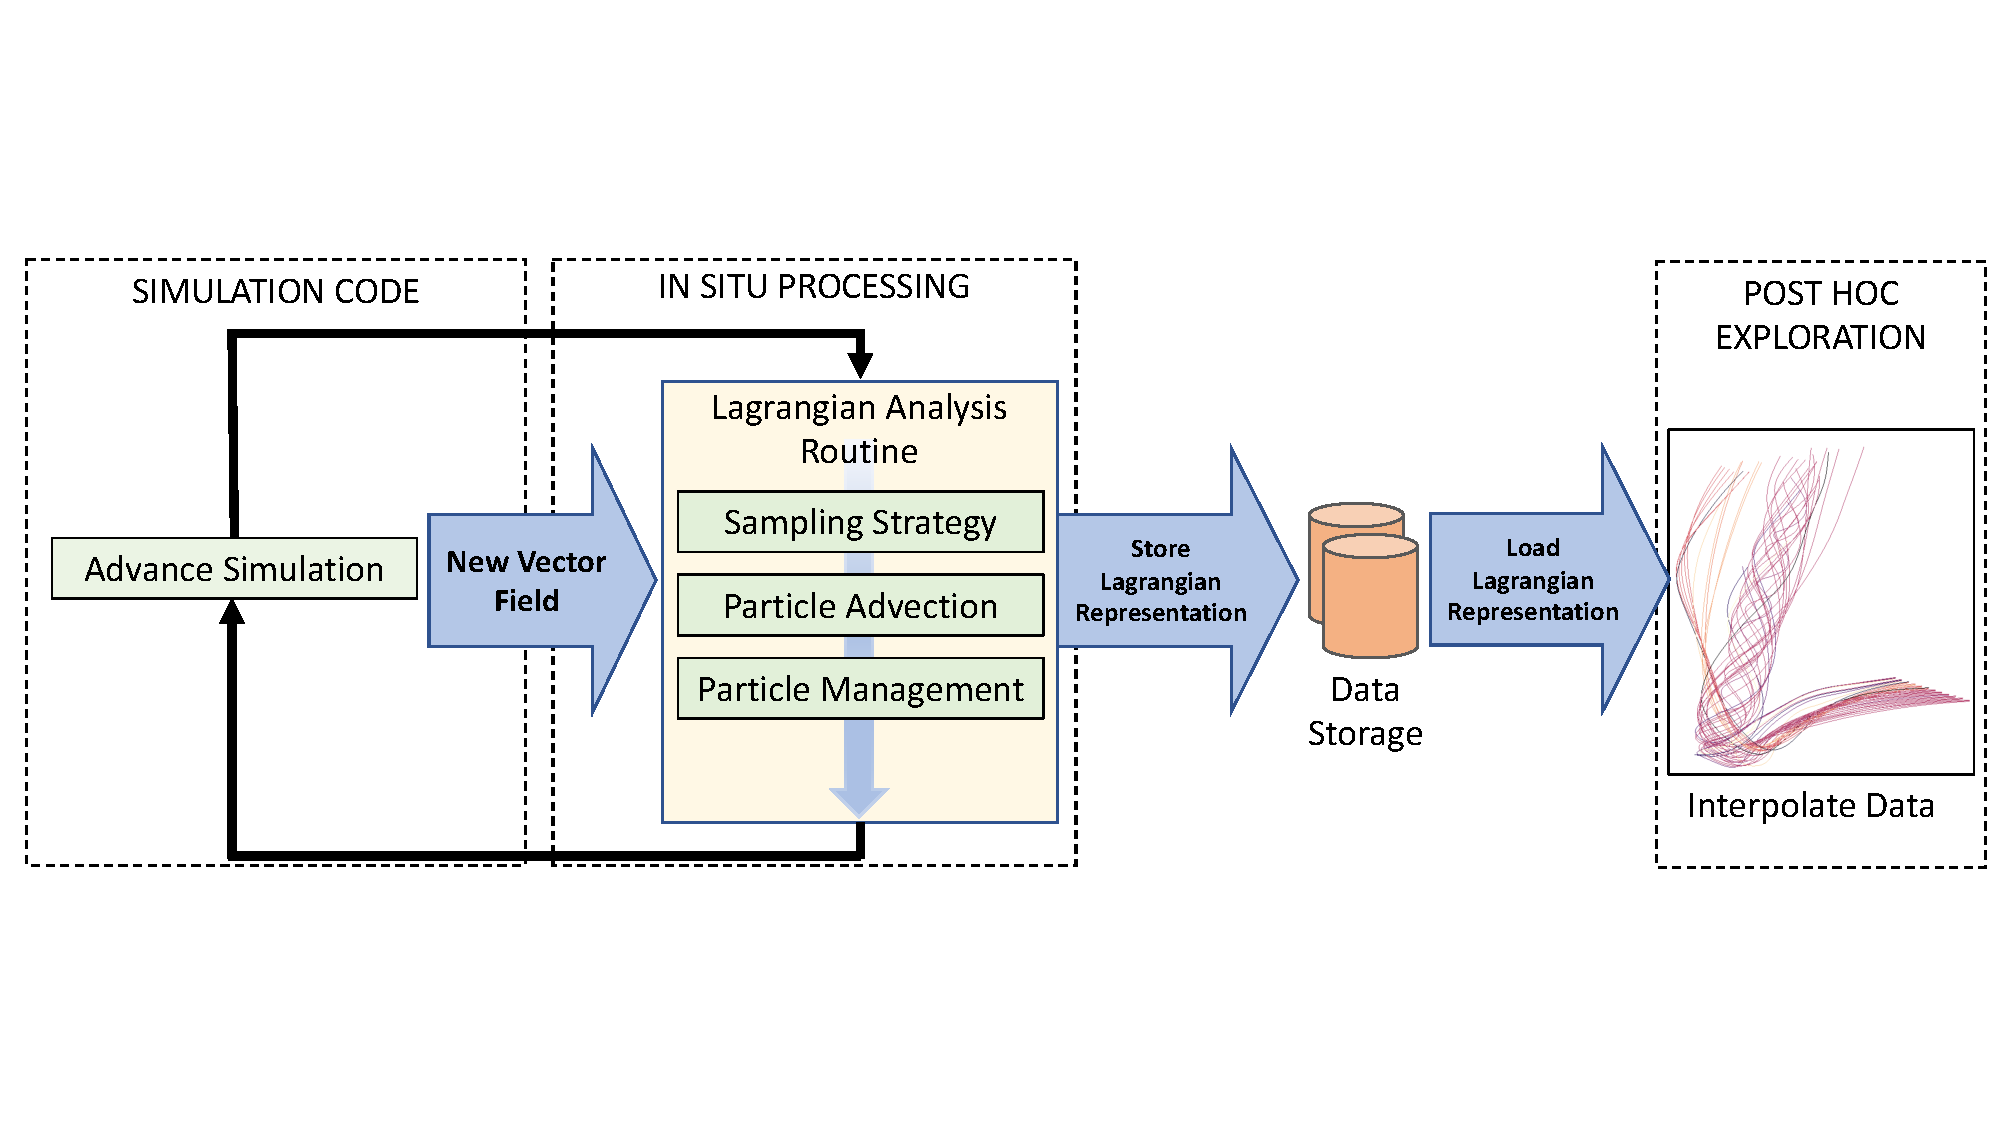
\includegraphics[width=0.9\linewidth,trim={0cm 4.3cm 0cm 4.3cm}, clip ]{Images/Schematic.pdf}
%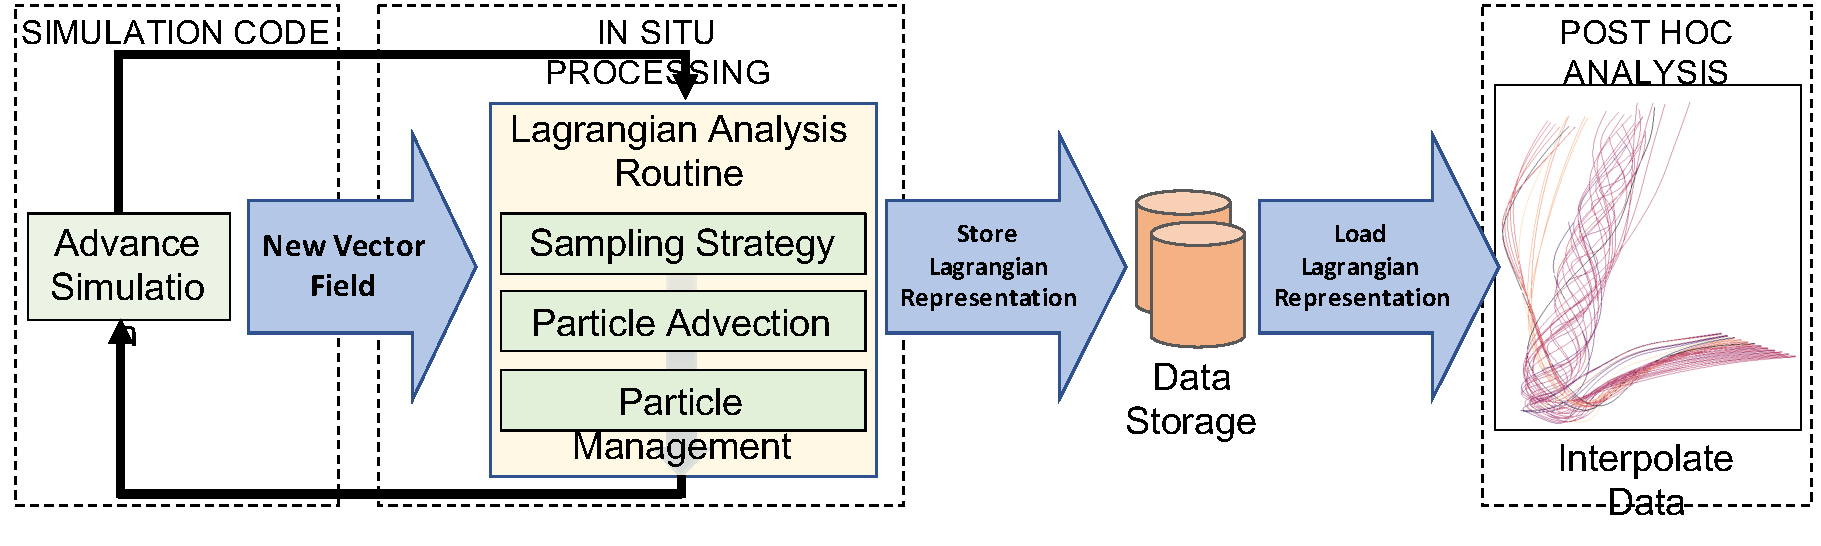
\includegraphics[width=0.9\linewidth]{Images/Schematic_Short.pdf}
\vspace{-2mm}
\caption{Schematic of the Lagrangian in situ reduction and post hoc exploration workflow.} %the simulation code with in situ processing integrated, data storage, and post hoc analysis.}
\vspace{-5mm}
\label{fig:schematic}
\end{figure}

%This section describes considerations for using and evaluating Lagrangian in situ reduction (L-ISR) for cosmology and seisomology time-varying vector fields. Specifically:
%\begin{tightItemize}
%\item Subsection~\ref{sec:instantiation} describes the instantiation we consider.
%\item Subsection~\ref{sec:evaluation} describes important evaluation criteria.
%\item Subsection~\ref{sec:workloads} describes important factors in defining workloads.
%\end{tightItemize}
%
%\subsection{Instantiation}
%\label{sec:instantiation}

This section describes the instantiation we consider for our study.
%
Figure~\ref{fig:schematic} shows a high-level description of the Lagrangian in situ reduction post hoc exploration (L-ISR-PHE) workflow. 
%
%There are many possible strategies for accomplishing the components within this workflow.
%
For our study, we focused on the current best practices in this space.
%
To describe our instantiation, the remainder of this section is divided based on the two phases: in situ reduction and post hoc exploration. 
%

\noindent\textbf{In Situ Reduction}
%In the in situ phase, for a data reduction operator without any a priori knowledge, a good strategy is to place samples such that domain coverage is maintained.
%
\fix{I love that you included this, but I think it is a distraction to
the reader.  Sadly, I propose you omit it.
}
Based on the in situ system classification in~\cite{childs2020terminology}, our L-ISR system classifies as one with a dedicated API integration, on node proximity, direct access, a time division of execution, automatic operation, and a derived output type.
%
\fix{Here is a possible replacement:
Both simulations we considered partitioned space amongst compute nodes,
with each compute node owning one portion of the vector field.
Our in situ routines followed this pattern, with an
instance of our Lagrangian analysis
routine running on each compute node, accessing its portion
of the vector field.
}
For our in situ data reduction strategy, we prioritized domain coverage.
\fix{I think the preceding sentence is a bit confusing.}
%
Similar to Agranovsky et al.~\cite{agranovsky2014improved}, we used uniform spatial sampling and a predetermined interval to store/reset particles.
%
Thus, we computed sets of temporally non-overlapping basis trajectories over the duration of the simulation.
%
%We refer to these trajectories as \textit{basis} trajectories.
%
Each set of basis trajectories encodes the behavior of the time-varying vector field over a specific interval of time.
%
%To introduce particles at the start of an interval, we use the uniform placement scheme by Agranovsky et al.~\cite{agranovsky2014improved}. 
%
%Using a uniform placement and resetting the particle trajectories after an interval helps maintain domain coverage and is simple to implement.
%
Our particle termination followed the local Lagrangian flow map model from Sane et al.~\cite{sane2020scalable}, where particles are terminated once they reach the end of the interval or exit the block.
%
Our implementation had two main knobs that control the total data storage and quality of reconstruction: number of basis trajectories, i.e., spatial sampling resolution, and frequency of storing information to disk, i.e., storage interval.
%
The effect of these settings varies depending on the underlying vector field. 
%
%We discuss these in~\ref{sec:workloads}.

We used the Ascent~\cite{Larsen2017Alpine} in situ infrastructure and VTK-m~\cite{moreland2016vtk} library to implement L-ISR. 
%
The Ascent API can be used to perform tightly-coupled integration with an application code and access various in situ analytics capabilities.
%%
The VTK-m Lagrangian filter on each rank operated independently and maintained its own list of particles.
%
We used the existing particle advection infrastructure available in VTK-m~\cite{pugmire2018performance}.
%
RK4 particle advection is implemented using VTK-m worklets (kernels) that offer performance portability by utilizing the underlying hardware accelerators.
%
In our implementation, each Lagrangian filter stored the displacement of each particle (three double), as well as its validity (one Boolean), i.e., whether the particle remained within the domain during the interval of calculation.
%
Overall, computing a Lagrangian representation increased the runtime memory cost on the simulation by approximately by four one-dimensional simulation ``fields''.
%
Simulations often have tens to hundreds of fields defined on the simulation grid, and thus, this cost would likely be acceptable for most simulations.
%
%In more complicated frameworks, it is possible to associate additional information (for example, ID, age, start location, previous locations, etc.) with each particle at the cost of higher runtime memory usage and data storage.
%

To compute a Lagrangian representation, the simulation invoked Ascent after every cycle it advanced.
%
Ascent accessed the simulation vector field data and consequently invoked the Lagrangian filter. 
%
The Lagrangian filter used the vector field to advance particles, and triggered the storage of trajectories at the end of an interval.
%
%In our implementation, following previous work~\cite{agranovsky2014improved}\cite{sane2018revisiting}\cite{sane2020scalable}, a trajectory in the Lagrangian representation is stored using a start and end location.
%
For integration, all the steps involved --- creating an instance of Ascent, specifying parameters, and invoking the VTK-m Lagrangian filter --- required only 23 lines of code (C++). % and less is a JSON input file was used.
%
%The code sample in Listing~\ref{lst:code} shows these steps. 
%

\noindent\textbf{Post Hoc Exploration}
For post hoc analysis, new particle trajectories are computed to explore the time-varying vector field. %by interpolating basis trajectories that were extracted in situ.
%
To construct new particle trajectories, we first identified which basis trajectories to follow and then performed interpolation.
%
Based on the study of accuracy of various Lagrangian-based advection schemes in~\cite{agranovsky2015subsampling}, our study employed a Delaunay triangulation to identify the neighborhood of valid basis trajectories and second-order barycentric coordinates for interpolation.
%
We used the CGAL~\cite{fabri2011cgal} library to construct and search the Delaunay triangulation.
%
After constructing new pathlines or deriving new scalar fields from the basis trajectories, we used VisIt~\cite{childs2012visit} to generate visualizations.

%\begin{lstlisting}[basicstyle=\footnotesize, label={lst:code}, caption=Ascent example., language=C++] 
%Ascent ascent;
%Node ascent_opts;
%ascent_opts[``runtime/type''] = ``ascent'';
%ascent.open(ascent_opts);
%conduit::Node mesh_data;
%conduit::Node pipelines;
%pipelines[``pl1/f1/type''] = ``lagrangian'';
%// filter knobs
%conduit::Node &lagrangian_params = pipelines[``pl1/f1/params''];
%lagrangian_params[``field''] = ``velocity'';
%lagrangian_params[``step_size''] = 0.02; 
%lagrangian_params[``storage_interval''] = 25; 
%lagrangian_params[``seed_resolution''] = 8; 
%conduit::Node actions;
%conduit::Node &add_pipelines = actions.append();
%add_pipelines[``action''] = ``add_pipelines'';
%add_pipelines[``pipelines''] = pipelines;
%conduit::Node &execute  = actions.append();
%execute[``action''] = ``execute'';
%conduit::Node &reset  = actions.append();
%reset[``action''] = ``reset'';
%ascent.publish(mesh_data);
%ascent.execute(actions);
%ascent.close();
%\end{lstlisting}
%
%
%We use Ascent to store the complete velocity field at a specified frequency in order to evaluate the traditional Eulerian paradigm.
%
%For every Eulerian configuration, we store the full spatial resolution of the simulation domain under consideration.
%

%\subsection{Evaluation Criteria}
%\label{sec:evaluation}
%In this study, we consider the following four evaluation criteria (EC) across the workflow:
%%
%\begin{tightEnumerate}
%\item\textbf{(EC1) In situ reduction time:} the execution time spent by the simulation on data analysis and visualization.
%\item\textbf{(EC2) In situ reduction memory:} the runtime memory used by in situ processing.
%\item\textbf{(EC3) Data storage size:} the file storage costs (i.e., bytes).
%\item\textbf{(EC4) Post hoc exploration accuracy:} the quantitative and qualitative accuracy of new interpolated trajectories or derived fields.
%\end{tightEnumerate}
%%
%
%\subsection{Workload Factors}
%\label{sec:workloads}
%To understand the performance characteristics of L-ISR, we identified four parameters that when varied produce the workloads we want to evaluate for our study:
%\begin{tightEnumerate}
%\item\textbf{(WF1) Number of basis particles:} 
%%We vary the number of basis particles initialized per rank. The number of basis trajectories impacts the cost of particle advection every cycle of the simulation, the size of the data stored to disk and the accuracy of the reconstruction. 
%%
%We specify the number of particles initialized using the notation $\textbf{1:X}$, where X is the reduction factor. For example, a 1:8 configuration states that one particle is used for every 8 grid points (12.5\% of the original data size). WF1 impacts every EC.
%\item\textbf{(WF2) Storage interval:} 
%%We consider the frequency at which files are stored to disk. Additionally, for the Lagrangian representation, the interval is equal to the integration length of each particle, and can thus, be consequential to the accuracy of reconstruction. 
%%
%We use $\textbf{I}$ to denote storage interval. WF2 impacts EC3 and EC4. 
%\item\textbf{(WF3) Grid size:} 
%%We consider different grid sizes to measure the in situ encumbrance of varying workloads. In particular, we are interested in the in situ encumbrance when a single compute node is operating on a large number of grid points. An additional benefit of varying the grid size is insight into the variation in simulation cycle time and consequently the percentage of time spent on in situ processing. 
%WC3 impacts EC1, EC2, and EC3. 
%\item\textbf{(WF4) Concurrency:} We consider the costs at multiple scales (i.e., number of compute nodes, MPI ranks). Further, the simulation codes described in \ref{sec:simulations} required different parallelization hardware, and thus, between simulation codes we measure the costs of Lagrangian representation extraction using, both, GPUs and CPUs for particle advection. WF4 impacts EC1 and EC2.
%\end{tightEnumerate}
